%2
\begin{frame}
  \begin{itemize}
    \item Cél: a nyers szöveg egyes részeit strukturálni, jelentésbeli többletet hozzáadni (pl. fejezetcím, bekezdés)
    \item Történeti előzmény: nyomdai előkészítés, kéziratok szerkesztése, gépi szedőrendszerek
    \item Példák jelölőnyelvekre: 
      \hiv{\href{http://man7.org/linux/man-pages/man7/roff.7.html}{roff}}, 
      \hiv{\href{https://www.latex-project.org/}{LaTeX}}, 
      \hiv{\href{https://en.wikipedia.org/wiki/Standard_Generalized_Markup_Language}{SGML}}
  \end{itemize}
\end{frame}

\subsection{roff}

%3
\begin{frame}
  \footnotesize
  \begin{description}[m]
    \item[RUNOFF] \hfill \\ nyers szövegből és parancsokból (.XX) álló fájlok $\to$ tördelt megjelenítés buta terminálokon (OS: Compatible Time Sharing System, CTSS, 1963)
    \item[runoff] \hfill \\ a RUNOFF bővített képességű portja \emph{IBM Selectric} terminálokhoz (OS: Multiplexed Information and Computing Service, multics, $\approx$'60-as évek vége)
    \item[roff] \hfill \\ a runoff továbbfejlesztése a Bell Telephone Labs-nál (1973) a PDP-11 géphez kapcsolt \emph{Graphic Systems CAT} (grafikus szedőegység) miatt. A roff család:
    \begin{description}[m]
      \item[troff] \hfill \\ typesetter roff a CAT-hez
      \item[nroff] \hfill \\ terminálokhoz és nyomtatókhoz
      \item[roff] \hfill \\ korlátozott képességű runoff utód, nem fejlesztették tovább
    \end{description}
    \item[groff] \hfill \\ GNU implementáció, máig fejlesztik $\to$ man oldalak
  \end{description}
\end{frame}

%4
\begin{frame}
  \begin{columns}[c]
    \column{0.5\textwidth}
      \tiny
      \begin{exampleblock}{\textattachfile{groff.1}{/usr/share/man/man1/groff.1.gz/groff.1}}
        \lstinputlisting[language=,breaklines=true,linerange={1-3},numbers=left,firstnumber=1]{groff.1}
        \lstinputlisting[language=,basicstyle=\ttfamily,breaklines=true,postbreak=\mbox{\textcolor{red}{$\hookrightarrow$}\space},linerange={75-85},numbers=left,firstnumber=75]{groff.1}
      \end{exampleblock}
    \column{0.5\textwidth}
      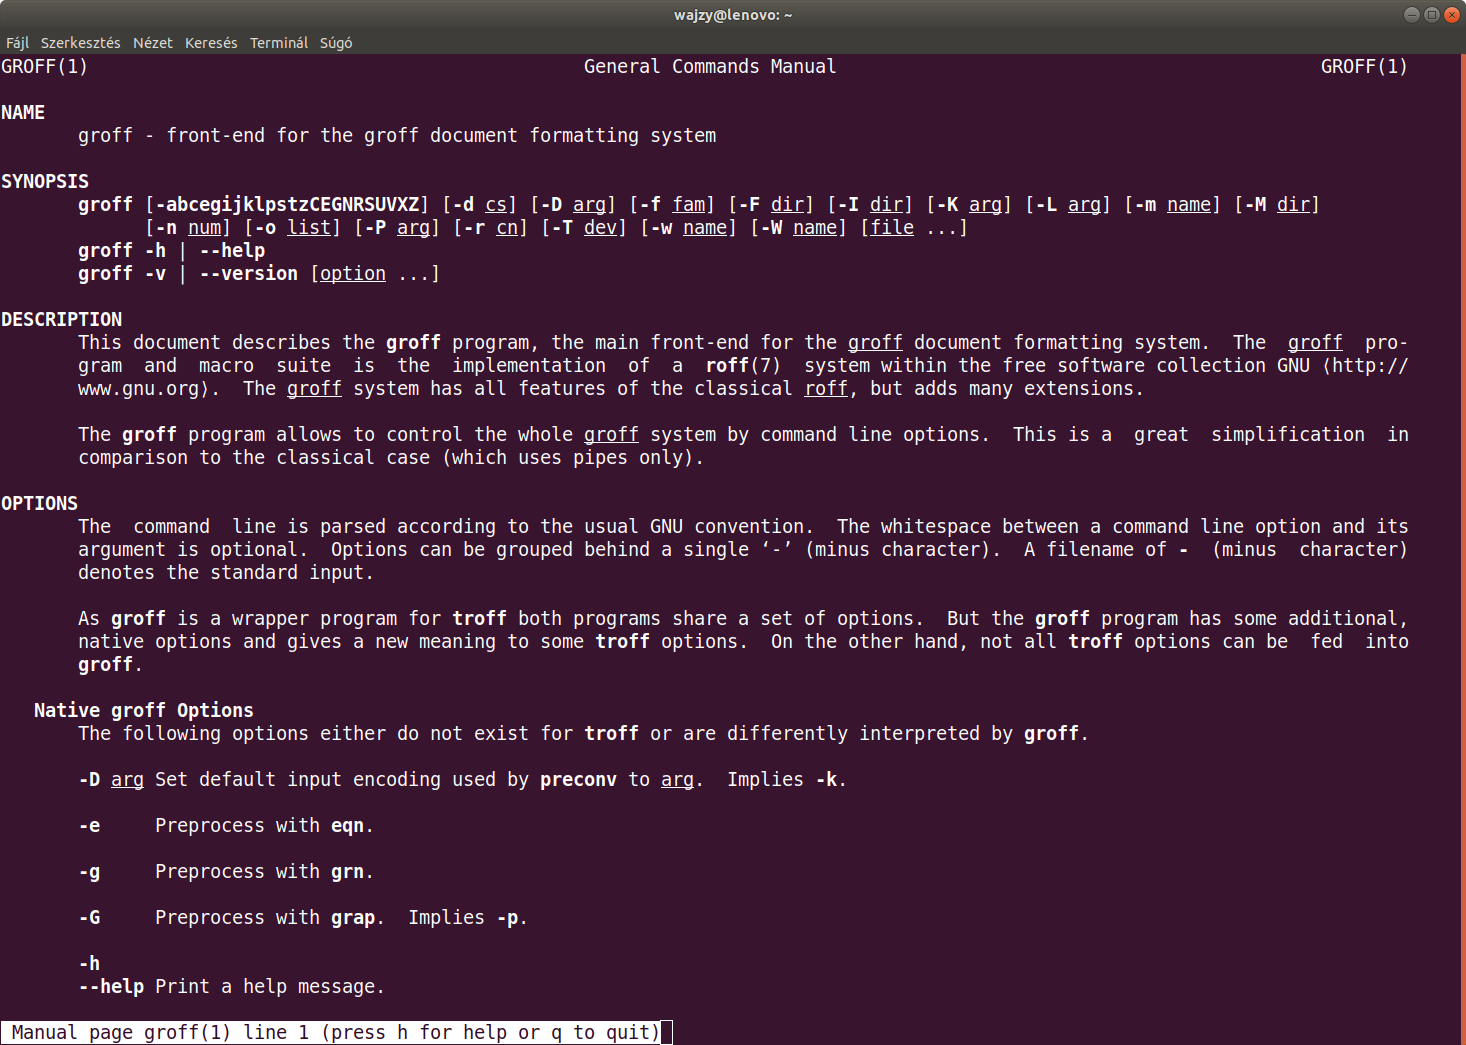
\includegraphics[width=\linewidth]{./groff.png}
  \end{columns}
\end{frame}

\subsection{\LaTeX{}}

%5
\begin{frame}
  \begin{columns}[T]
    \column{0.3\textwidth}
      \begin{description}[m]
        \item[\TeX] \hfill \\ Betűszedő rendszer, fejlesztője Donald E. Knuth, 1978 (Elégedetlenség \hiv{\href{https://www-cs-faculty.stanford.edu/~knuth/taocp.html}{könyvének}} szedésével.)
        \item[\LaTeX] \hfill \\ \TeX-en alapuló szövegformázó rendszer, Leslie Lamport, 1983
      \end{description}
    \column{0.7\textwidth}
        \begin{exampleblock}{\textattachfile{html1.tex}{html1.tex}}
          \centering
          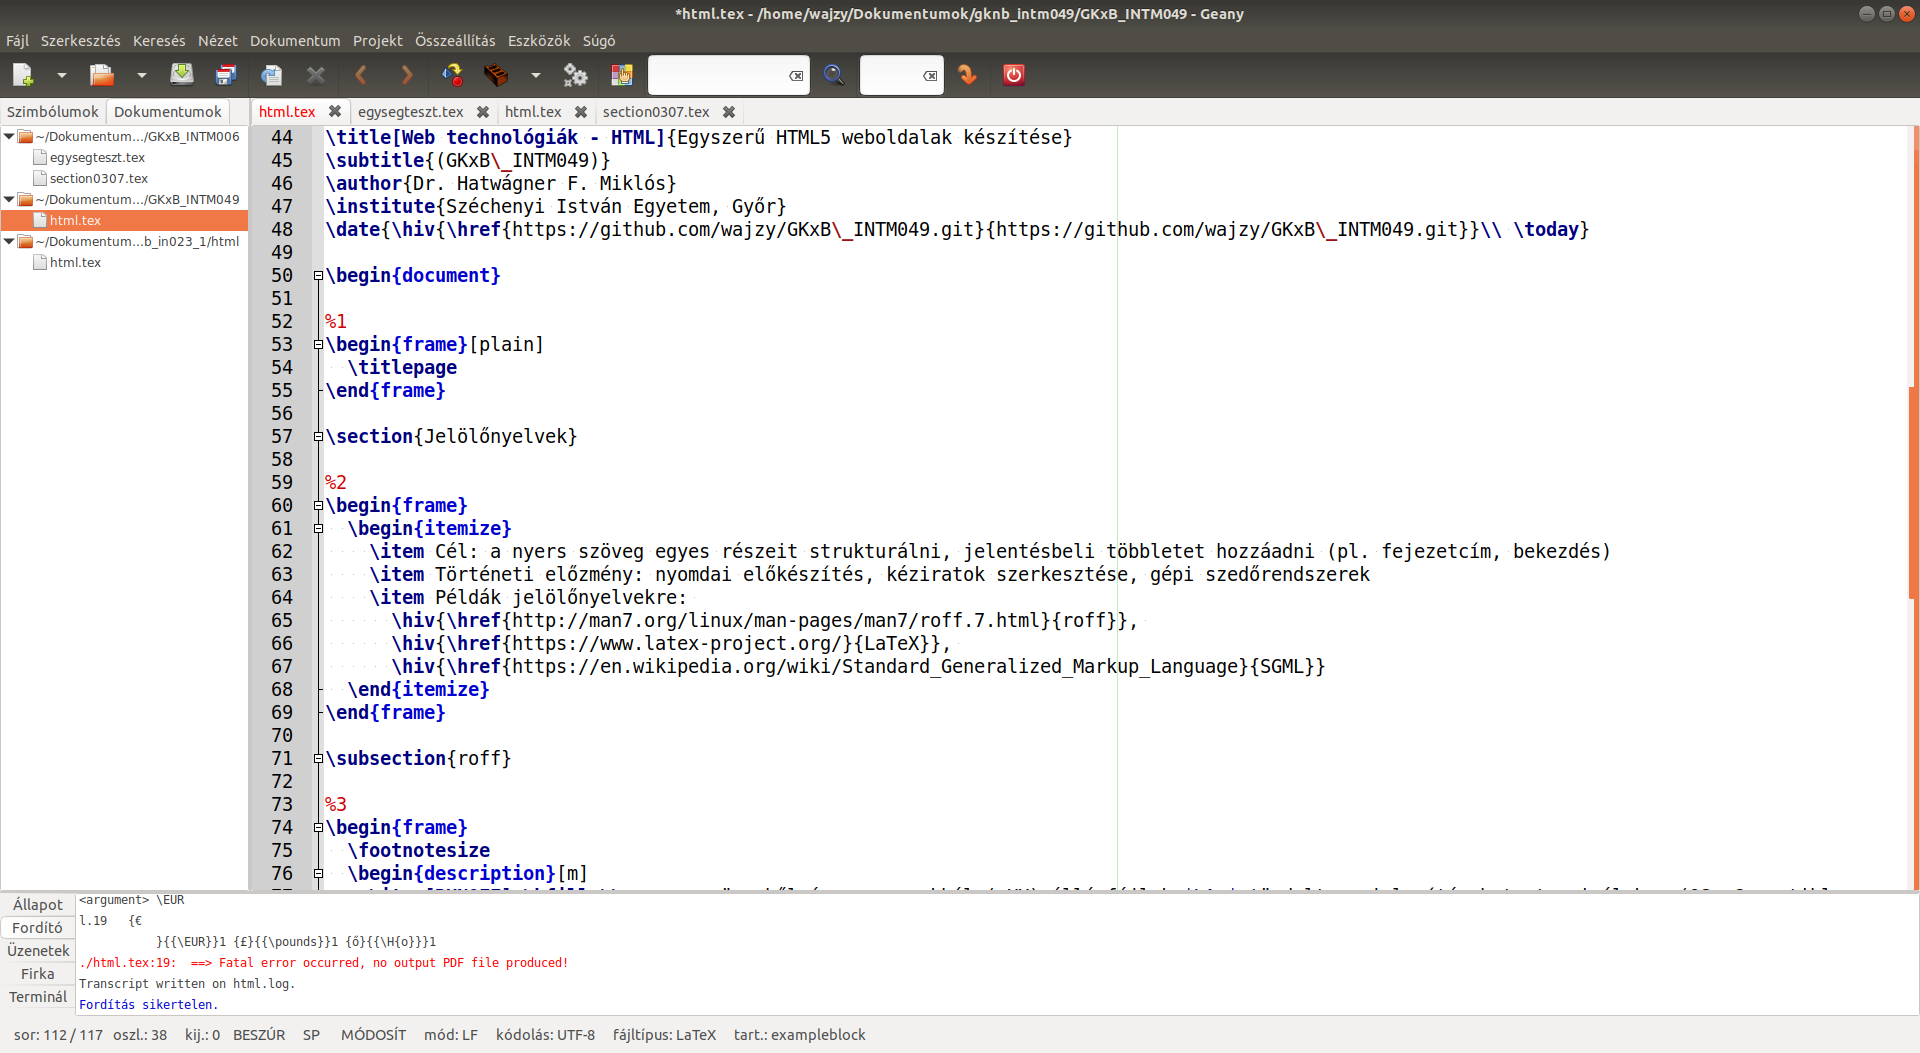
\includegraphics[scale=.14]{./latex.png}
        \end{exampleblock}
  \end{columns}
\end{frame}

\subsection{SGML}

%6
\begin{frame}
  \begin{itemize}
    \item SGML (Standard Generalized Markup Language), ISO 8879:1986
    \item Szabványos jelölőnyelv dokumentumok szerkezetének leírására,
beleértve a címkék definiálását is
    \item Gépfüggetlen metanyelv
    \item Előzménye: GML (1969)
    \begin{itemize}
      \item C. \kiemel{G}oldfarb (IBM), E. \kiemel{M}osher, R. \kiemel{L}orie
      \item dokumentumtípusonként egyedi kódolási séma definiálható
      \item előre definiált elemek egymásba ágyazhatóak
      \item először az IBM nyomdarendszere használta
    \end{itemize}
    \item Tulajdonságai
    \begin{itemize}
      \item Deklaratív: struktúrát és attribútumokat rögzít, nem a feldolgozás módját ($\to$~időtállóság)
      \item Gépi feldolgozás lehetősége
    \end{itemize}
  \end{itemize}
\end{frame}

%7
\begin{frame}
  \begin{itemize}
    \item Legfontosabb építőelemek
    \begin{itemize}
      \item Elemek ([element] nyitó és záró cimkék [tag] által határolva)
      \item A nyitó tagben attribútumok (kulcs-érték párok) adhatók meg
      \item Elemek egymásba ágyazhatóak
      \item Elemek, attribútumok alkalmazási szabályai $\to$ Document Type Definition (DTD)
    \end{itemize}
    \item Néhány korai, jelentős alkalmazás
    \begin{itemize}
      \item Electronic Manuscript Project of the Association of American Publishers (AAP, tudományos dokumentumok)
      \item Computer-aided Acquisition and Logistic Support (CALS, katonai dokumentumok kezelése)
      \item LinuxDoc (Linux csomagok)
    \end{itemize}
  \end{itemize}
\end{frame}

%8
\begin{frame}[fragile]
  \scriptsize
  \begin{columns}[T]
    \column{0.4\textwidth}
    \begin{exampleblock}{SGML példa}
      \begin{verbatim}
<!DOCTYPE PEOPLE SYSTEM 
  "people.dtd">
<PEOPLE DATE="15 6 2000">
 <NAME TITLE="Mr">
  <FIRST>Wally</FIRST>
  <LAST>Wallpaper</LAST>
 </NAME>
 <NAME>
  <LAST>Jackson</LAST>
 </NAME>
 <NAME TITLE="Dr">
  <FIRST>Susan</FIRST>
  <MIDDLE>Ramsay</MIDDLE>
  <LAST>Sukie</LAST>
 </NAME>
</PEOPLE>
\end{verbatim}
    \end{exampleblock}
    \column{0.6\textwidth}
    \begin{exampleblock}{people.dtd}
      \begin{verbatim}
<!ELEMENT people - - (name+)>
<!ATTLIST people date NUMBERS #REQUIRED>

<!ELEMENT name - - (first?, middle?, last)>
<!ATTLIST name title CDATA #IMPLIED>

<!ELEMENT first - - (#PCDATA)>
<!ELEMENT middle - - (#PCDATA)>
<!ELEMENT last - - (#PCDATA)>
\end{verbatim}
    \end{exampleblock}
    \tiny
    Forrás: \textattachfile{chap4.html}{OmniMark dokumentáció}
  \end{columns}
\end{frame}

\subsection{A HTML története}

%9
\begin{frame}
  \begin{itemize}
    \item ENQUIRE: a CERN dokumentumtároló, -megosztó szoftvere. (Tim Berners-Lee, 1980)
    \item HTML első említése: T.B.L., 1991 (18 elem, melyek a CERN SGMLguid-on, a kutatóintézet SGML alkalmazásán alapultak)
    \item A HTML egy SGML alkalmazás: 1993-2014
    \item HTML 4.01: Strict/Transitional/Frameset DTD, 1999
    \item Aktuális változat: \hiv{\href{https://www.w3.org/TR/html52/}{HTML5}}
    \item Néhány újdonság: videó- és hanglejátszás, vektorgrafika, többszálúsítás, helyi adattárolás, bittérképes grafika, stb.
    \item ,,Élő szabvány'', meghatározó szervezetek: \hiv{\href{https://www.w3.org/}{W3C}} (ajánlások), \hiv{\href{https://whatwg.org/}{WHATWG}} (innovatív technológiák)
    \item 2019-től a WHATWG tartja karban a HTML szabványát.
    \item XHTML: XML előírásoknak megfelelő HTML; a HTML5 ,,feleslegessé'' tette
  \end{itemize}
\end{frame}
